\chapter{Sprint 1 : Authentification et gestion des utilisateurs}\label{chap4}

\section{Introduction}

Le premier sprint est consacré à l'identification des utilisateurs et au contrôle d'accès. L'objectif est de permettre l'inscription, la connexion par jeton de session, l'authentification Google et la gestion des profils selon trois rôles.

\section{Objectifs du sprint}

\begin{itemize}
    \item Mettre en place l'inscription et la connexion sécurisée.
    \item Générer un jeton de session stocké sous forme de hash dans la base.
    \item Intégrer Google OAuth pour le web et le mobile.
    \item Distinguer les rôles patient, médecin et administrateur.
    \item Réaliser les interfaces de connexion, d'inscription et de paramètres.
\end{itemize}

\section{Backlog du sprint}

\begin{table}[H]
\centering
\begin{tabular}{|p{3cm}|p{6cm}|p{2cm}|p{3cm}|}
\hline
\textbf{User story} & \textbf{Description} & \textbf{Priorité} & \textbf{Critère d'acceptation} \\
\hline
US1 --- Inscription & Créer un compte patient & Haute & Compte créé et profil patient associé \\
\hline
US2 --- Connexion & S'authentifier avec email et mot de passe & Haute & Jeton retourné et redirection selon le rôle \\
\hline
US3 --- Rôles & Restreindre les routes selon le rôle & Haute & Accès refusé pour un rôle non autorisé \\
\hline
US4 --- Profil & Modifier ses informations personnelles & Moyenne & Modification enregistrée \\
\hline
\end{tabular}
\caption{Backlog du sprint 1}
\end{table}

\section{Authentification par jeton}

La Figure \ref{fig:auth_seq} décrit le déroulement d'une connexion. Le mot de passe est vérifié côté backend, puis un jeton aléatoire est généré ; seul son hash SHA-256 est conservé dans \texttt{SessionToken}. Le profil utilisateur est mis en cache dans Redis pour accélérer les requêtes suivantes.

\begin{figure}[H]
\centering
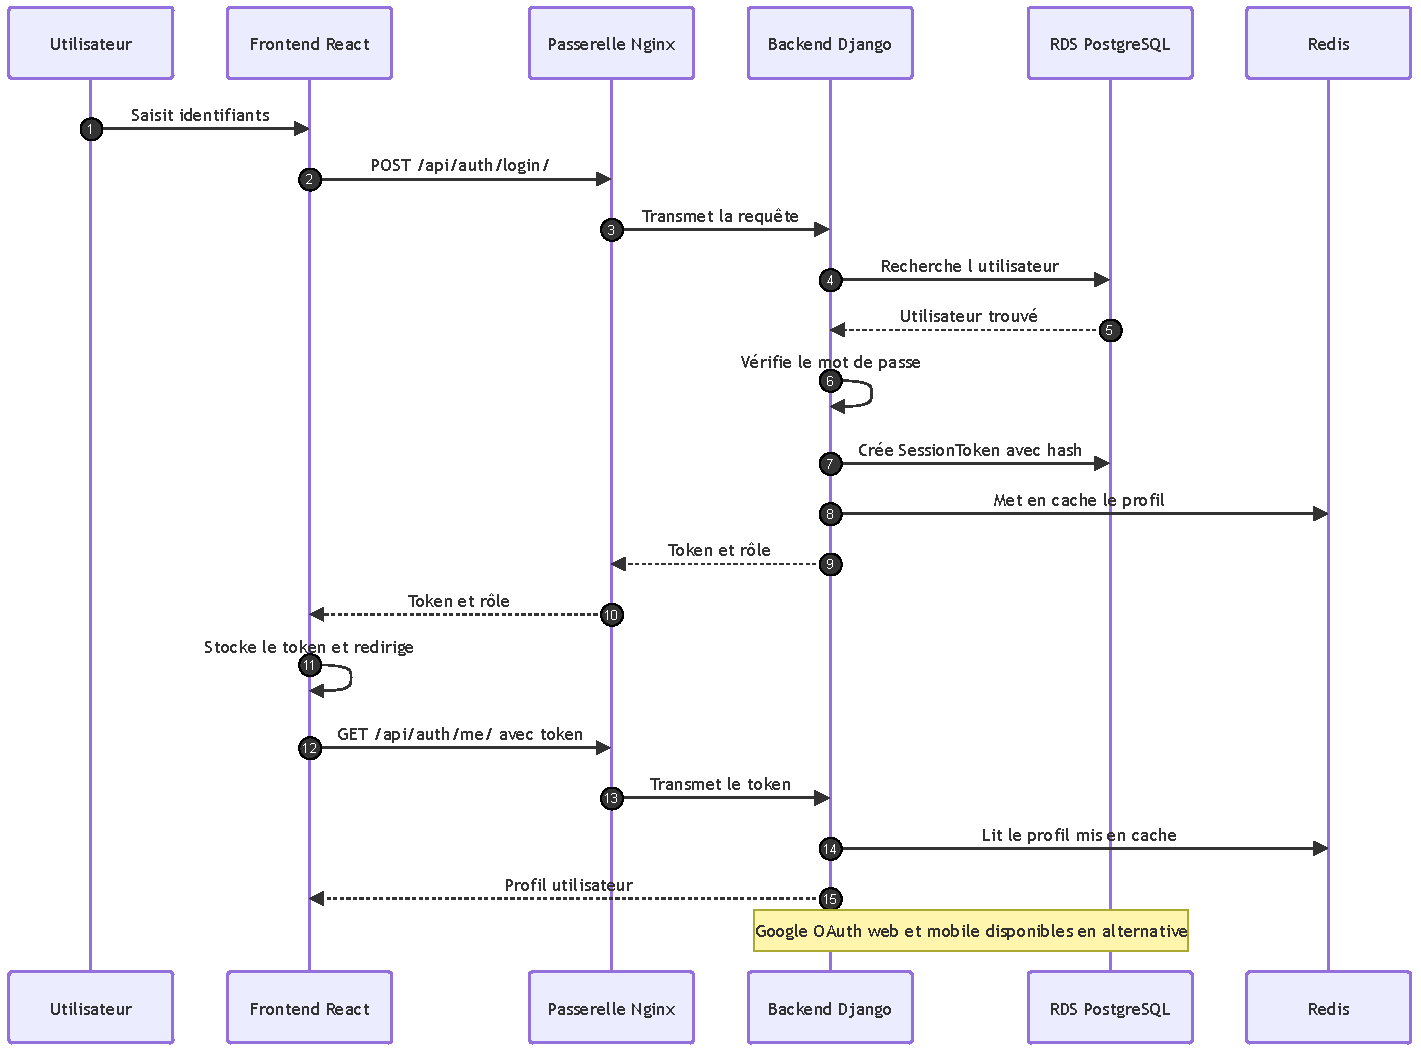
\includegraphics[width=\textwidth]{06-authentification-sequence.pdf}
\caption{Séquence d'authentification par jeton}
\label{fig:auth_seq}
\end{figure}

\section{Contrôle d'accès}

Le contrôle d'accès repose sur deux mécanismes complémentaires : la vérification du rôle pour les opérations sensibles et le filtrage des requêtes selon l'appartenance des données. Un médecin ne voit ainsi que les épisodes dont il est le praticien, et un patient uniquement les siens. Les refus sont journalisés dans \texttt{AuditLog}.

\section{Réalisation}

La Figure \ref{fig:login_screen} présente la page de connexion et la Figure \ref{fig:register_screen} la page d'inscription.

\begin{figure}[H]
\centering
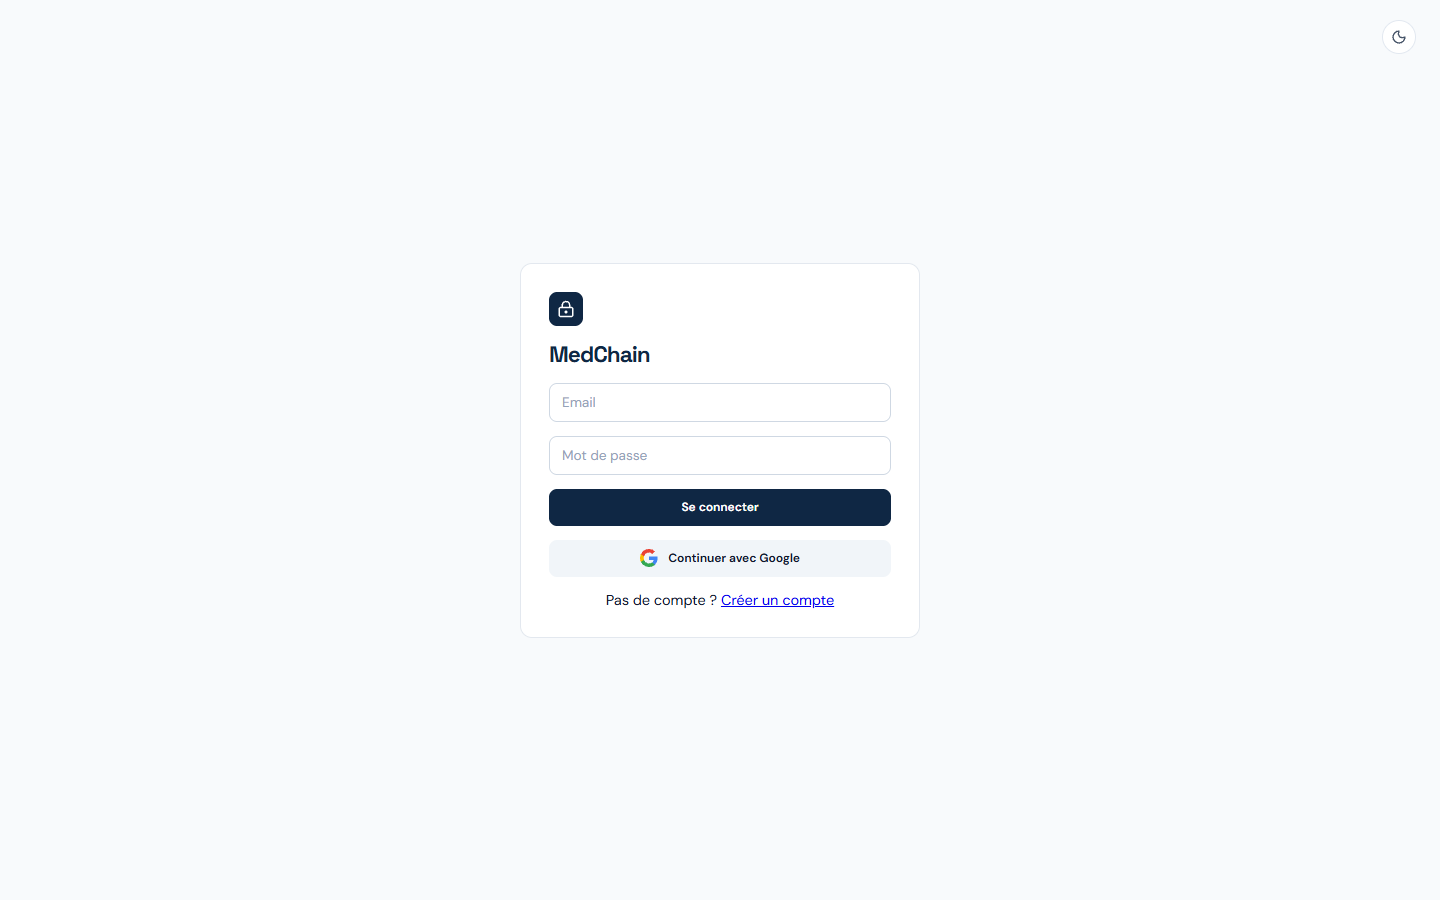
\includegraphics[width=0.8\textwidth]{S02-connexion.png}
\caption{Interface de connexion}
\label{fig:login_screen}
\end{figure}

\begin{figure}[H]
\centering
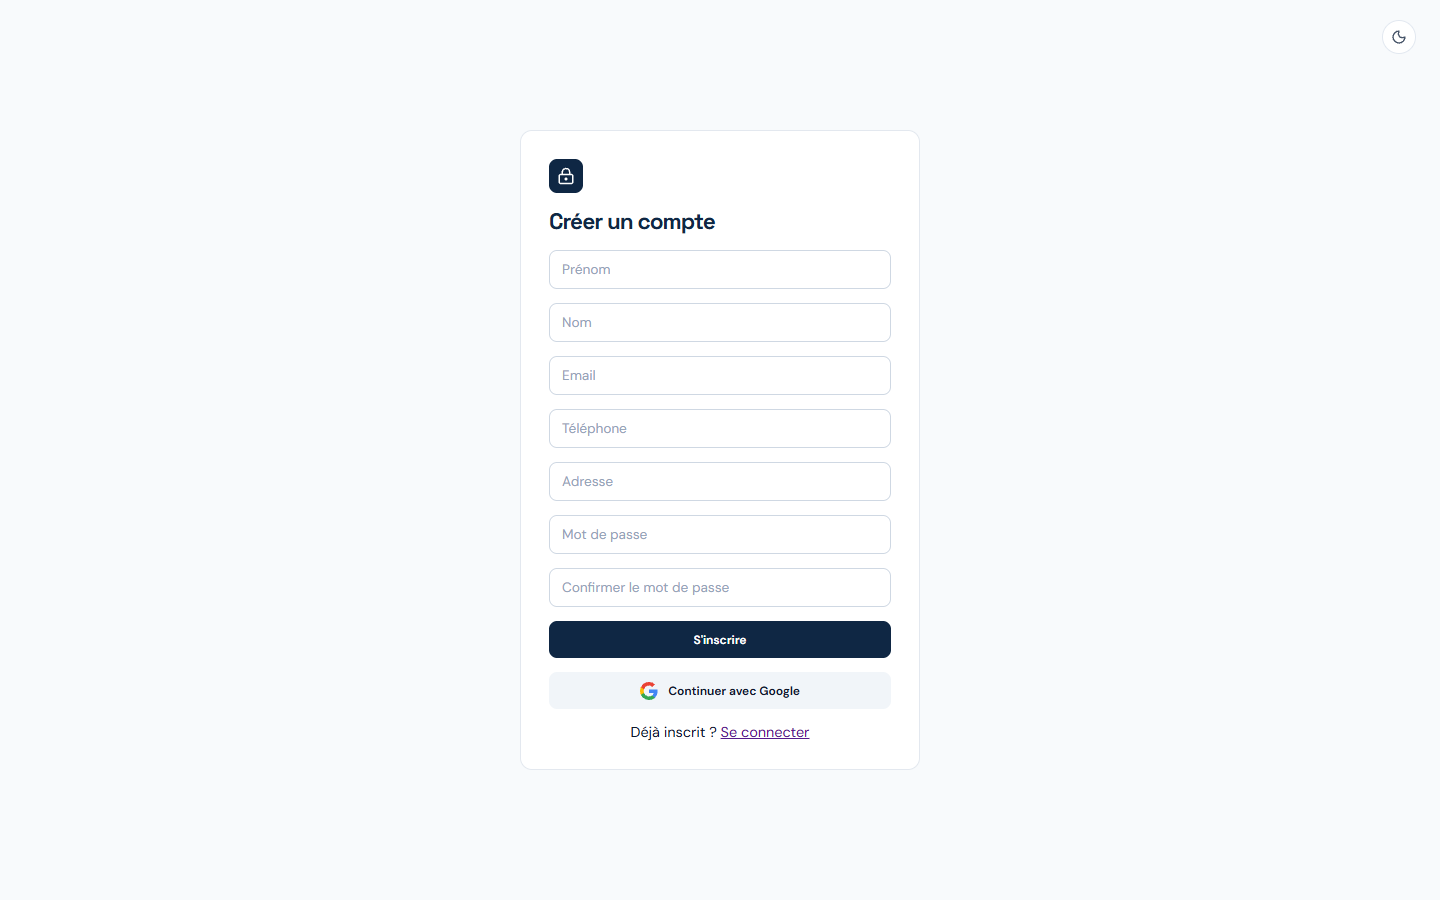
\includegraphics[width=0.8\textwidth]{S03-inscription.png}
\caption{Interface d'inscription}
\label{fig:register_screen}
\end{figure}

La Figure \ref{fig:settings_screen} montre la page de paramètres du compte et la Figure \ref{fig:admin_screen} le tableau de bord réservé à l'administrateur.

\begin{figure}[H]
\centering
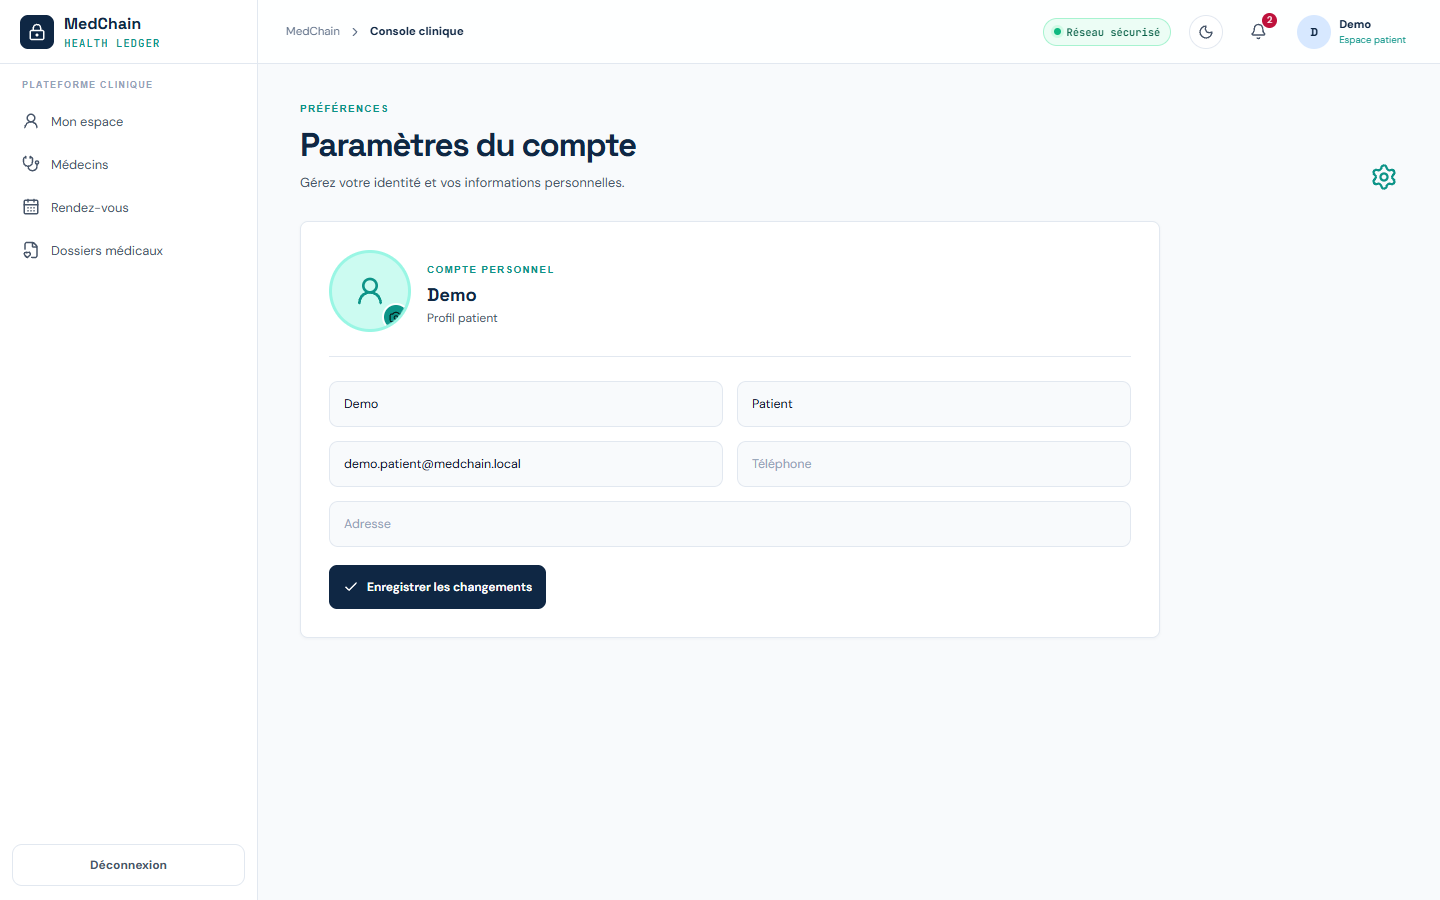
\includegraphics[width=\textwidth]{S10-parametres.png}
\caption{Paramètres du compte}
\label{fig:settings_screen}
\end{figure}

\begin{figure}[H]
\centering
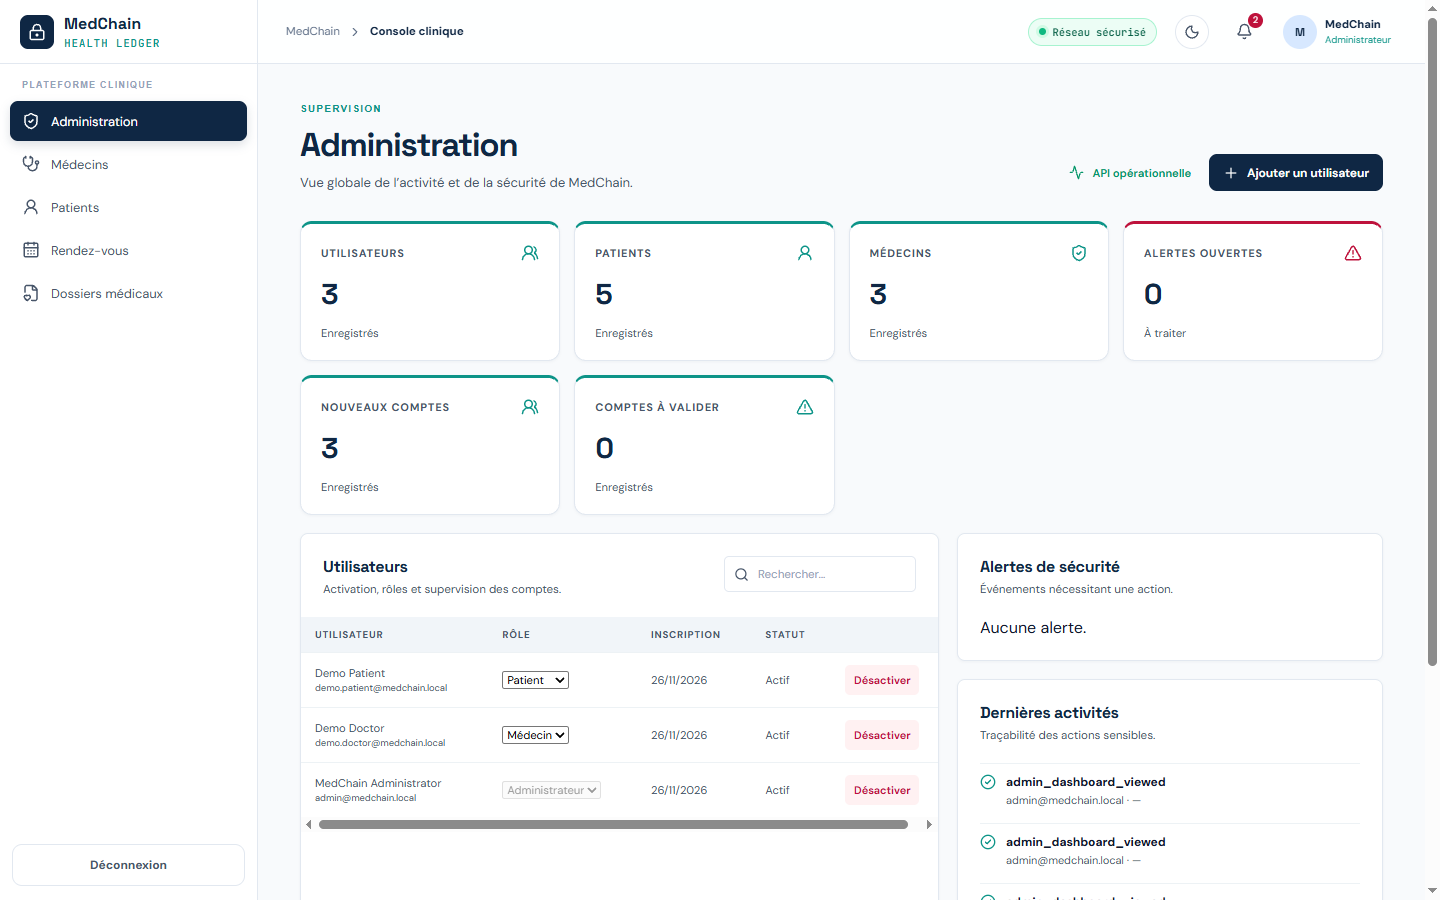
\includegraphics[width=\textwidth]{S14-tableau-administrateur.png}
\caption{Tableau de bord administrateur}
\label{fig:admin_screen}
\end{figure}

\section{Conclusion}

À l'issue de ce sprint, l'authentification, la gestion des rôles et la supervision des comptes sont opérationnelles. Le sprint suivant porte sur le parcours de soins et la traçabilité des traitements.
